\chapter{Privacy for Smart Contracts}
\section{Introduction}
\begin{center}
	\begin{figure}
		\centering
		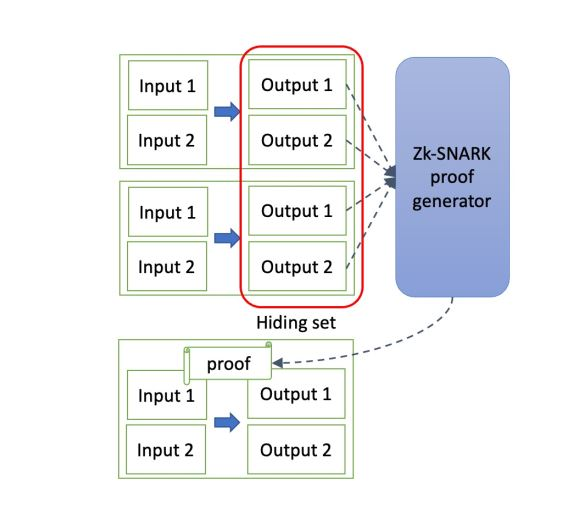
\includegraphics[width=0.8\linewidth]{Fig/20/F1}
		\caption{UTXO model was introduced in Bitcoin. However, it leads to information leakage. Zcash employs zk-SNARKs to shield the information on the payment’s origin, destination, or amount in a payment transaction.}
		\label{fig:L20_f1}
	\end{figure}
\end{center}
In the preceding lecture, we delved into the utilization of Zcash to introduce privacy within a UTXO state management system. This model involves transactions comprising inputs and outputs, with outputs specifying recipients' public keys and inputs referencing prior outputs. However, this UTXO framework inadvertently leaks information, allowing transactions to be linked together, forming a graph. Zcash presents a comprehensive framework to address this issue, ensuring that payment transactions maintain privacy by concealing their origin, destination, and amount. Refer to Figure \ref{fig:L20_f1} for a visual representation of this concept.\\
\begin{center}
	\begin{figure}
		\centering
		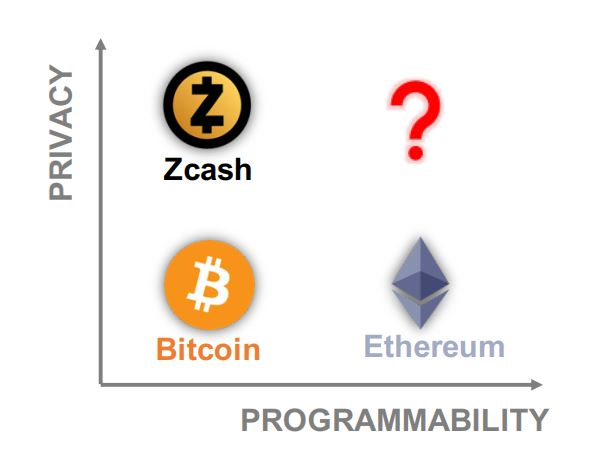
\includegraphics[width=0.8\linewidth]{Fig/20/F2}
		\caption{Bitcoin offers neither privacy nor programmability. It avails simple scripts that can be used for writing only the payment transactions. On the other hand, Zcash offers complete privacy but no programmability. In contrast to that, Ethereum offers high degree of programmability but no privacy. Currently, there is no deployed blockchain ecosystem that offers both privacy and programmability.
		}
		\label{fig:L20_f2}
	\end{figure}
\end{center}
While the UTXO model is straightforward, its inherent simplicity restricts on-chain programming for intricate computations requiring state information or multiple participants, as depicted in Figure \ref{fig:L20_f2}. To overcome these limitations, Ethereum adopts an account-based model, facilitating programmability through the execution of smart contracts within the Ethereum Virtual Machine (EVM). This advancement has led to the emergence of various financial tools like decentralized exchanges, arbitrage, flash loans in decentralized finance (DeFi), tokenization, and games on the Ethereum platform.\\
However, contemporary account-based blockchain systems suffer from a lack of privacy, as all transaction details are public. For instance, consider an account that acquires Ether from a cryptocurrency exchange such as Coinbase, utilizes it for executing an arbitrage opportunity (as shown in Figure \ref{fig:L20_f3}), and subsequently converts the Ether to a fiat currency like USD. Due to the transparency of Ethereum transactions, the cryptocurrency exchange becomes privy to the real-world identity of the entity that engaged in the arbitrage.\\
\begin{center}
	\begin{figure}
		\centering
		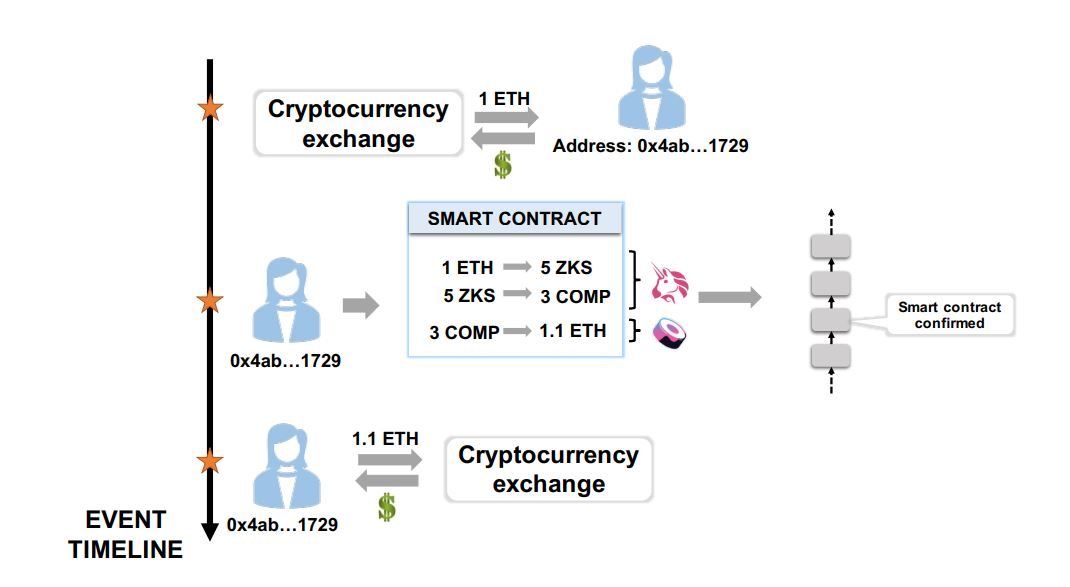
\includegraphics[width=0.8\linewidth]{Fig/20/F3}
		\caption{An entity buys Ether from a cryptocurrency exchange such as Coinbase. Then, using smart contract, it successfully executes an arbitrage opportunity that involves exchanging Ether for ZKS and ZKS for COMP in Uniswap and then, COMP for Ether in Sushiswap. After that, the entity exchanges the Ether for USD in Coinbase. However, Coinbase has full access to the real-world  identity of this entity (through the "know your customer" (KYC) process).
		}
		\label{fig:L20_f3}
	\end{figure}
\end{center}
Drawing from our previous study of Zcash, a pertinent question arises: Can we apply zk-SNARKs to safeguard the internal transaction details within an account-based ecosystem like Ethereum? A successful design in this context would harmonize privacy and programmability. However, before addressing this question, we must clarify the notion of transaction privacy. A transaction internally comprises various elements, including sender and recipient addresses, transaction value, exchanged tokens, utilized liquidity pools, timestamps, and more. Therefore, transaction privacy may entail concealing specific combinations of these components, such as sender and recipient addresses, while leaving others accessible to the public eye, see Figure \ref{fig:L20_f4}. This lecture ventures into a construction that ensures this level of privacy, referred to as user privacy. In this construct, information about the transaction's value and tokens exchanged remains discernible, while the identities of the involved accounts remain shielded.
\begin{center}
	\begin{figure}
		\centering
		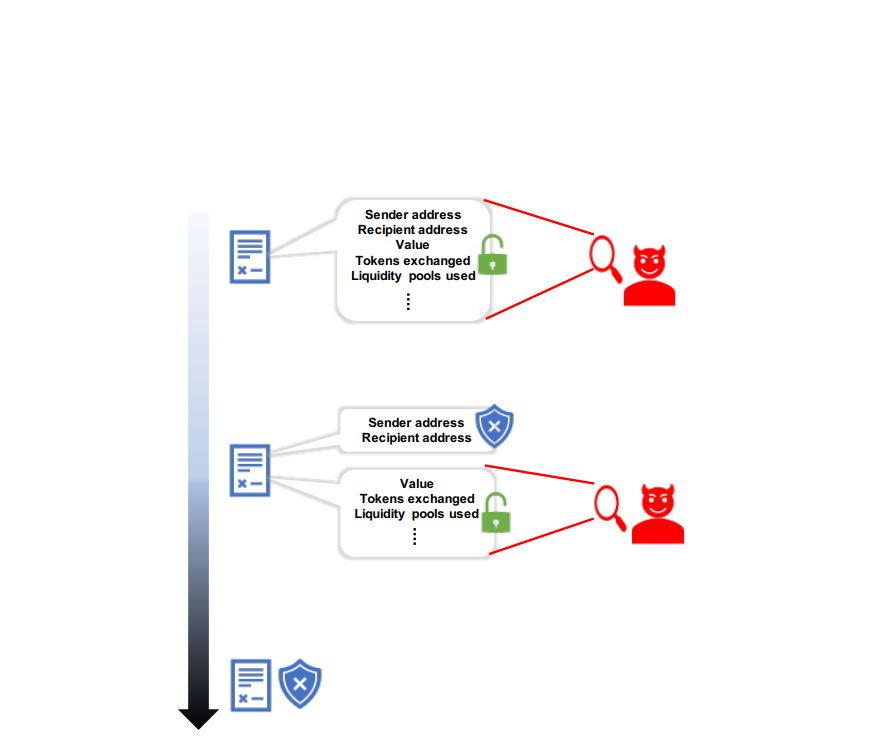
\includegraphics[width=0.8\linewidth]{Fig/20/F4}
		\caption{In the initial scenario, every aspect of the transaction is openly accessible to the public. This mirrors the current privacy state observed in Ethereum and similar blockchain ecosystems based on smart contracts. A modest degree of privacy enhancement can be attained by concealing solely the sender's and recipient's addresses within the transaction. The pinnacle of privacy is achieved when every component of a transaction is cloaked, yet the transaction itself remains auditable and verifiable.
		}
		\label{fig:L20_f4}
	\end{figure}
\end{center}
\section{Key Idea}
The fundamental concept to achieve user privacy within an account-based blockchain ecosystem involves leveraging a privacy-preserving blockchain such as Zcash as a foundation. In this context, a participating node necessitates an account within Ethereum to facilitate various activities like payment transactions and DeFi trading. There exist two viable methods by which an account can execute transactions while preserving privacy:\\
\begin{enumerate}
	\item \textbf{Indirect Liquidity Injection via Zcash:} The node can begin by acquiring a privacy-preserving token, such as Zcash, from a cryptocurrency exchange using fiat currency. Subsequently, utilizing Zcash's hiding set, the node can introduce liquidity into its Ethereum account. By employing this hiding set, any potential linkage between the Zcash account (which obtained tokens from the exchange) and the Ethereum account is severed.
	\item \textbf{Asset Movement through Flash Loans:} Another approach entails the node securing a flash loan from liquidity pools such as Aave within an Ethereum account. The node can then transfer this asset to a Zcash account, leveraging Zcash's hiding set to transfer the asset back to a different Ethereum account. This method similarly severs links between transactions conducted on Ethereum and the accounts utilized by the node for liquidity.
\end{enumerate}
In both scenarios, the transactions executed on Ethereum remain visible to entities like cryptoexchanges or liquidity pools. However, these entities lack the means to establish connections between the trades and the specific accounts employed by the node for liquidity purposes. If a node desires to prevent other nodes from associating its transactions with its accounts, the node can again utilize Zcash's hiding set to disrupt these connections, as outlined above (refer to Figure \ref{fig:L20_f5}). It is important to note that while external parties, such as cryptoexchanges and liquidity pools, can observe Ethereum transactions, they are unable to ascertain the precise identity of the node engaged in these transactions. This approach effectively safeguards user privacy.\\
\textbf{Utilize a privacy-preserving}\\
By employing the concept of a hiding set, the node can effectively obscure any links between its activities in different blockchain ecosystems, ensuring that transactions and accounts remain untraceable.\\
Here's a summarized breakdown of the steps:
\begin{enumerate}
	\item \textbf{Acquiring Tokens and Creating Accounts:} The node establishes an account within a privacy-preserving blockchain like Zcash and acquires tokens through an exchange using fiat currency. The limited programmability of Zcash does not impact the node's ability to hold and transfer these tokens.
	\item \textbf{Utilizing the Hiding Set:} The node employs the hiding set mechanism to generate a new account in the target blockchain ecosystem, such as Ethereum. This hiding set serves to mask any connection between the Zcash account and the new Ethereum account, ensuring privacy.
	\item \textbf{Smart Contract Engagement:} With the new account established, the node can create or interact with smart contracts on Ethereum, enabling a wide range of activities such as arbitrage, swaps, payment transactions, and more. These activities are conducted within the smart contract's execution, keeping the node's identity and actions private.
	\item \textbf{Asset Conversion:} When the node decides to convert its tokens back to fiat currency like USD, it utilizes the hiding set once again. This step involves transferring the assets from the Ethereum smart contract to another Zcash account, effectively breaking any link between the Ethereum smart contract and the Zcash account.
	\item \textbf{Exchange to Fiat Currency:} With the tokens safely in the Zcash account, the node exchanges them for fiat currency on a cryptoexchange. The link between the Ethereum smart contract and the Zcash account remains hidden, preserving privacy.
	\item \textbf{Link Masking Across Transactions:} The same strategy of utilizing the hiding set can be employed by the node to mask links between different transactions performed from its accounts in Ethereum. This ensures that no external observer can trace and connect these transactions to the node's identity.
\end{enumerate}
By following these steps, the node effectively safeguards its privacy across various blockchain ecosystems, using the privacy-preserving features of Zcash and the hiding set mechanism to obscure connections and maintain anonymity.
\begin{center}
	\begin{figure}
		\centering
		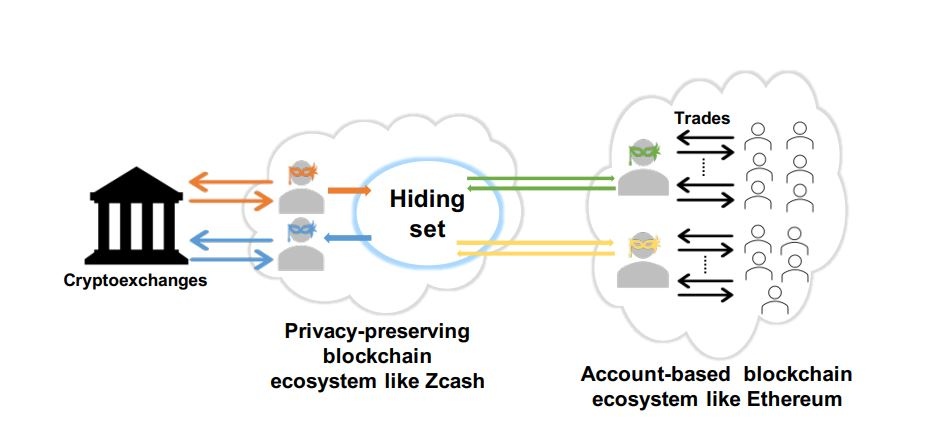
\includegraphics[width=0.8\linewidth]{Fig/20/F5}
		\caption{
			how a node can utilize a privacy-preserving blockchain like Zcash to achieve user privacy in an account-based ecosystem like Ethereum.
		}
		\label{fig:L20_f5}
	\end{figure}
\end{center}
In a privacy-preserving blockchain like Zcash, some of the input and output UTXOs in a  transaction can be shielded and some of the other input and output UTXOs can be public.
\begin{center}
	\begin{figure}
		\centering
		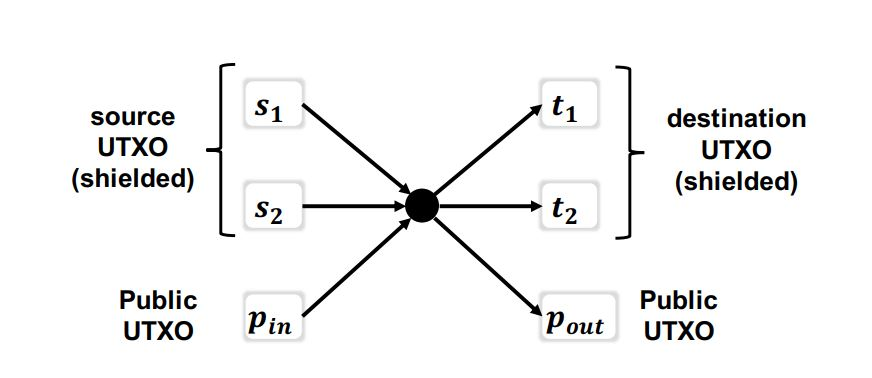
\includegraphics[width=0.8\linewidth]{Fig/20/F6}
		\caption{
			In a privacy-preserving blockchain like Zcash, some of the input and output UTXOs in a  transaction can be shielded and some of the other input and output UTXOs can be public.
		}
		\label{fig:L20_f6}
	\end{figure}
\end{center}
\section{Construction}
We can establish a privacy bridge to smart contracts by harnessing the unique privacy features of Zcash, allowing for a seamless integration of a privacy-preserving side and a programmability side within a single blockchain framework, see Figure \ref{fig:L20_f6}. In this construction, transactions are strategically designed to maintain privacy while enabling complex smart contract executions.\\
\begin{center}
	\begin{figure}
		\centering
		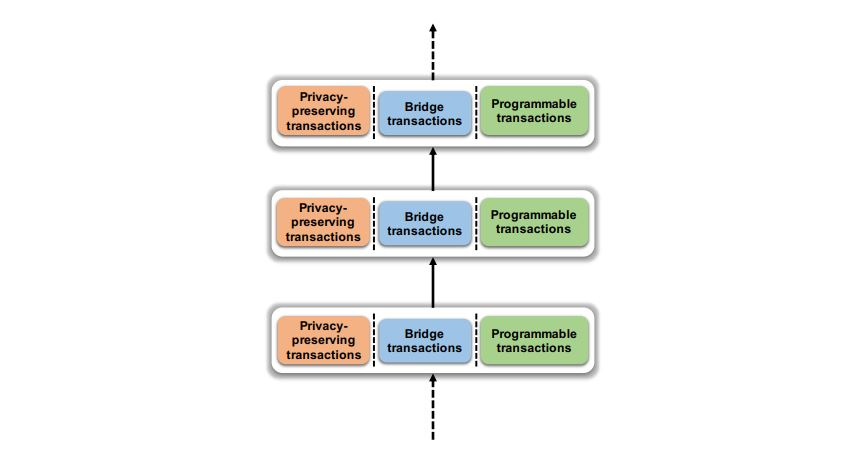
\includegraphics[width=0.8\linewidth]{Fig/20/F7}
		\caption{
			Each block can contain three types of transactions - privacy-preserving transactions, bridging transactions and programmable transactions.
		}
		\label{fig:L20_f7}
	\end{figure}
\end{center}
\begin{center}
	\begin{figure}
		\centering
		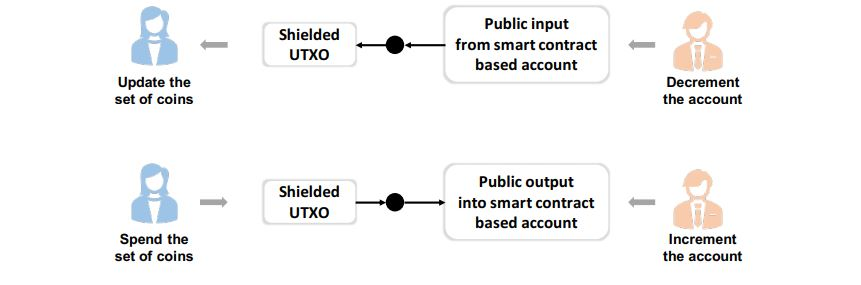
\includegraphics[width=0.8\linewidth]{Fig/20/F8}
		\caption{
			Pictorial illustration of the two types of bridging transactions: the first one decreases the assets/tokens in the account of the smart contract and atomically outputs shielded UTXOs in the privacy-preserving side, the second one involves spending unspent UTXOs in the privacy -preserving side and outputting a public output that increments the account of the smart contract in the programmability-side. Both these transactions must be executed atomically.
		}
		\label{fig:L20_f8}
	\end{figure}
\end{center}
The privacy bridge operates through a two-fold mechanism, with distinct sides offering specific functionalities. Participants are assigned an address on the privacy-preserving side, adhering to the UTXO model. Transactions occurring entirely within this side, involving senders and recipients with addresses on the UTXO model of the privacy-preserving side, enjoy inherent privacy and are termed "privacy-preserving transactions", see Figure \ref{fig:L20_f7}. However, for intricate operations necessitating programmability, funds can be transferred from the privacy-preserving side to smart contracts on the programmability side through intermediary "bridging transactions."\\
On the programmability side, nodes can utilize smart contracts to execute "programmable transactions" for implementing complex strategies. Notably, these programmable transactions do not conceal details like the addresses of involved smart contracts, exchanged tokens, or transaction value. The privacy-preserving transactions and the publicly viewable programmable transactions coexist within this side, each serving its specific purpose.\\
Two types of bridging transactions facilitate the movement of assets between the two sides, while maintaining privacy, see to Figure \ref{fig:L20_f8}:
\begin{enumerate}
	\item \textbf{Type One Bridging Transaction:} This type involves decrementing tokens in the programmability side and generating a shielded UTXO in the privacy-preserving side, which updates the associated coin holdings while preserving the privacy of the source account.
	\item \textbf{Type Two Bridging Transaction:} Here, a UTXO from the privacy-preserving side is spent to increment tokens in the specified smart contract on the programmability side.
\end{enumerate}
These bridging transactions are executed seamlessly, ensuring atomicity. Consequently, a single block can accommodate three transaction types: privacy-preserving transactions, bridging transactions, and programmable transactions, see Figure \ref{fig:L20_f7}.\\
In essence, while smart contracts execute diverse strategies on the programmability side, the bridging transactions act as a shield, preventing the exposure of addresses from the privacy-preserving side that initiated the smart contract's funding, or the addresses involved in the asset transfer to the privacy-preserving side, see Figure \ref{fig:L20_f9}. As a result, the privacy of accounts within the privacy-preserving side remains intact, impervious even to scrutiny from entities like cryptocurrency exchanges such as Coinbase.
\begin{center}
	\begin{figure}
		\centering
		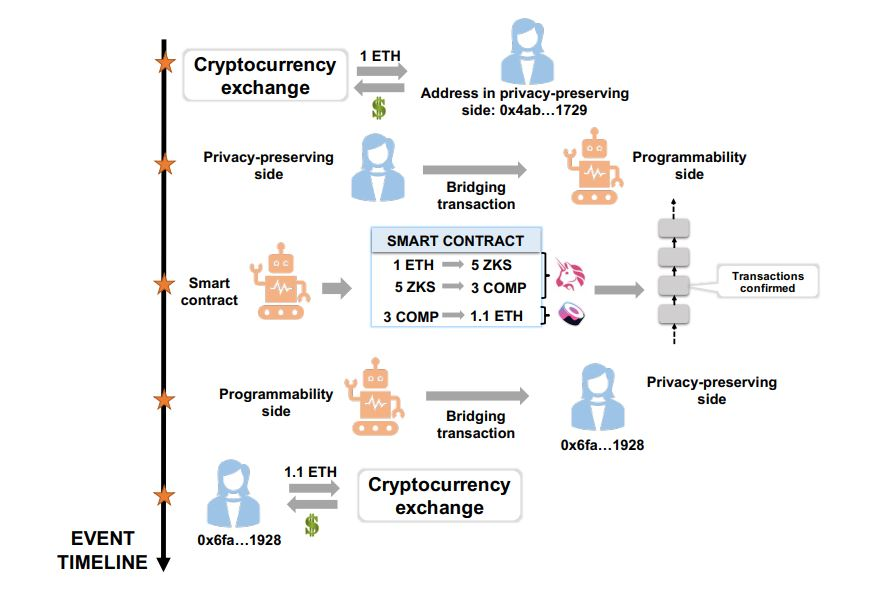
\includegraphics[width=0.8\linewidth]{Fig/20/F9}
		\caption{
			Privacy bridge preserves the privacy of the addresses in the privacy-preserving side that funded and received assets from the smart contract in the programmability-side.
		}
		\label{fig:L20_f9}
	\end{figure}
\end{center}
\section{References}
In this lecture we saw a simple technique to harness the Zcash architecture on UTXOs to smart contract platforms. This bridging technique brings user privacy, but the actual contents of the transaction (such as the amounts) are public. A more general technique would shield such data; even more generally, perhaps all data on the blockchain could be encrypted and yet be validated by the participants. Such a broad goal is tantamount to true \href{https://en.wikipedia.org/wiki/Homomorphic_encryption}{homomorphic encryption}, which refers to computing on encrypted data without the need for any secret key, a grand goal of cryptography. Several recent works have attempted to build such general privacy preserving architectures: \href{https://eprint.iacr.org/2018/962.pdf}{zexe}, \href{https://eprint.iacr.org/2019/191}{Zether}, \href{https://github.com/eth-sri/zkay}{zkay}, \href{https://eprint.iacr.org/2020/543}{kachina}, and this is an active area of research and development.\\
zexe is a ledger-based system where users can execute offline computations while hiding all information about the computations and subsequently produce transactions, attesting to the correctness of these computations which can be validated in constant time. Zether is a smart contract in Ethereum that keeps the account balances encrypted and exposes methods to deposit, transfer and withdraw funds to/from accounts through cryptographic proofs. zkay is a language formalism which introduces privacy types for Solidity. kachina is a framework for deploying privacy-preserving smart contracts under the Universal Composition (UC) model.